\chapter{PROPOSED WORK}

\noindent{We propose a decentralized solution using blockchain technology and IPFS. The programmable blockchain we are using is Ethereum. Using ethereum we try to ensure that the certificates once issued are further immutable. \\

Storing data over the blockchain is expensive, to facilitate this we use another distributed network called IPFS to store all the details of the users. This has advantages over the centralized storages in a way that, no single node has control over all the data. It also maintains versioning and any change made to the data can be traced back. The CID obtained from the IPFS is stored over the blockchain, thus uniform datatype of fixed memory can be defined in the smart contract.\\

For the process of validation, the data available with the user is checked if present on the blockchain and then certifcate is produced by accessing data from the IPFS. 
}

\section{Architecture}
\subsection{Admin Module}

    \begin{itemize}
        \item Issuing authority is authenticated via login portal.
        \item Issuer collects child’s data and pushes it to IPFS.
        \item IPFS returns a hash which is saved in local Db. and the issuer uses this hash and makes a transaction into the ethereum blockchain.
        \item The transaction is validated using a PoW consensus algorithm and verified by other fellow peers.
        \item Then the transaction hash\_id is returned to the issuer.
        \item This hash\_id is then mailed to the respective parent.
    \end{itemize}

    \begin{figure}[H]
        \centering
        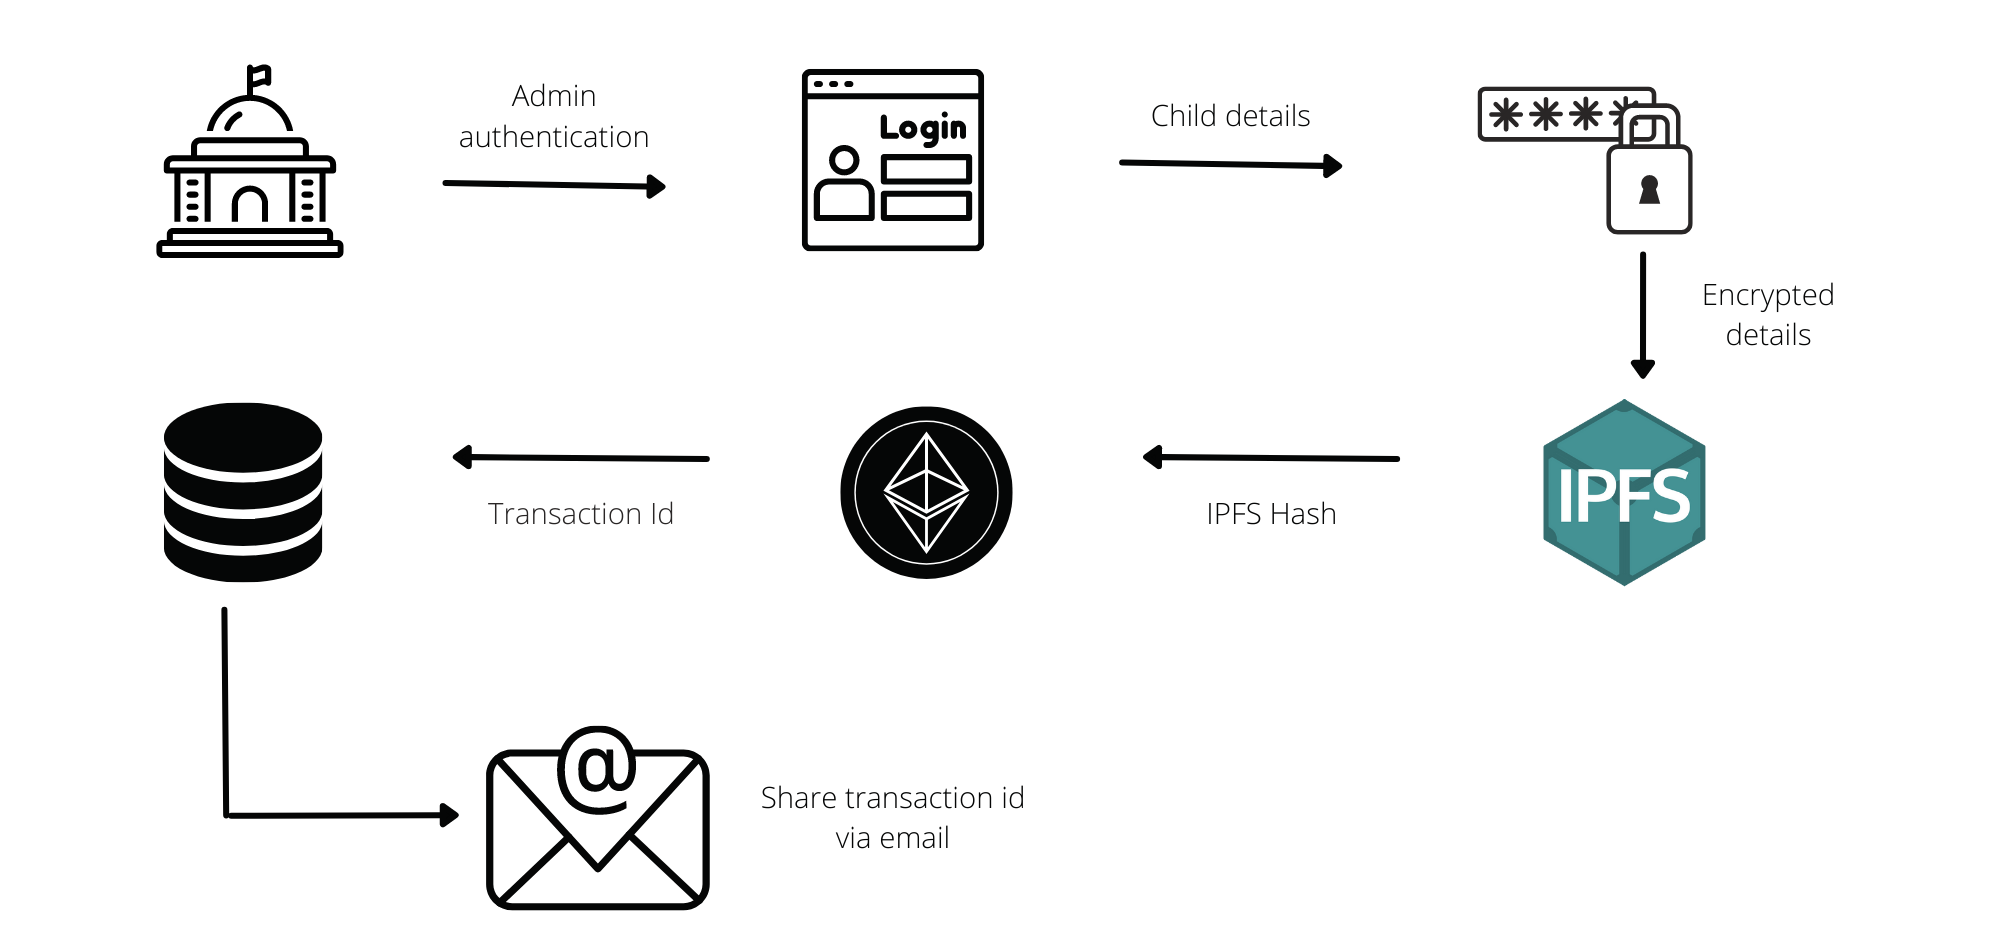
\includegraphics[width=\textwidth]{imgs/Admin_module.png}
        \caption{Admin module of the project}
        \label{fig:Admin module of the project}
        \end{figure}

\subsection{Client Module}
        \subsubsection{Parent/Child}

        \begin{itemize}
            \item Parents/Child login into the platform using the hash id and registration no. given via mail.
            \item On clicking the view/verify certificate, a call is made to the ethereum blockchain and hash\_id is passed as argument.
            \item If the hash\_id is not present in the chain, the certificate does not exist.
            \item If it is present , the details are shown to the user and ipfs hash is retrieved from the chain. 
            \item Using ipfs hash the details of the certificate are retrieved from ipfs network and shown to the user in the form of certificate.
        \end{itemize}
    
        \begin{figure}[H]
            \centering
            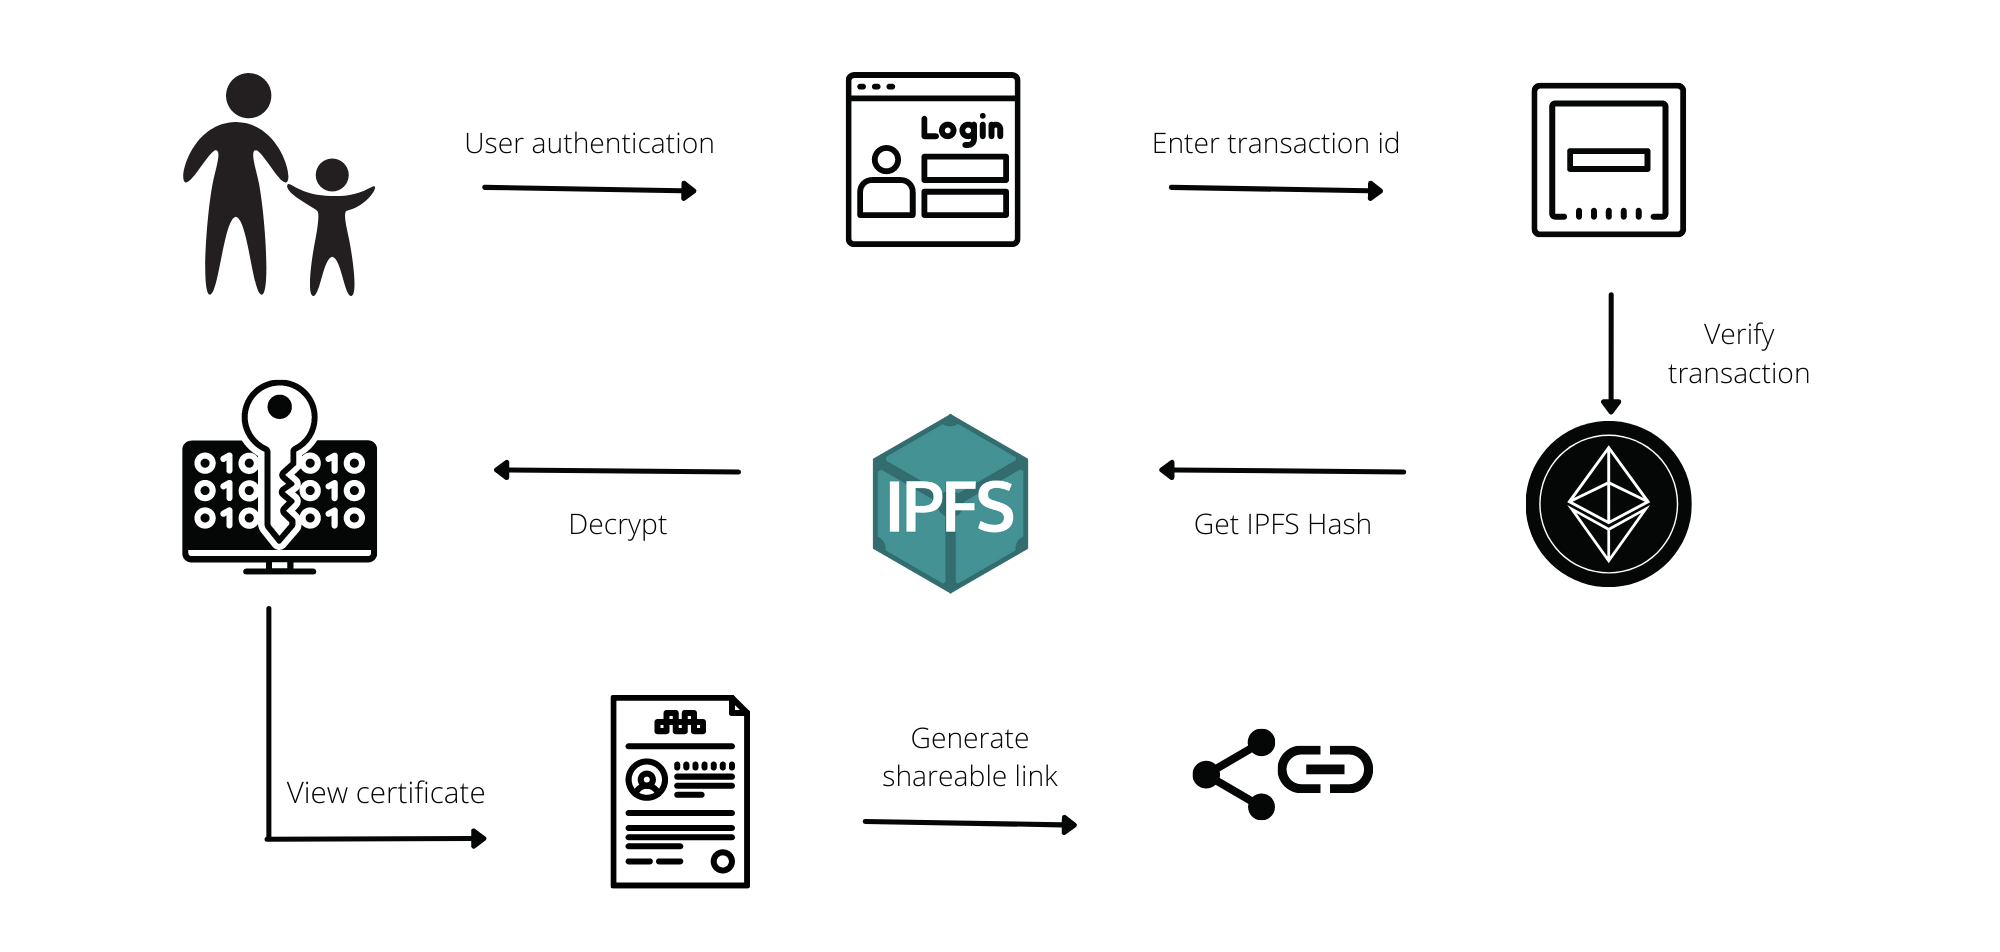
\includegraphics[width=\textwidth]{imgs/Child_Parent_module.png}
            \caption{Child/Parent module of the project}
            \label{fig:Child/Parent module of the project}
            \end{figure}

    \subsubsection{Third Party where document is shared}

        \begin{itemize}
            \item Parent/Child can share a temporary link to the third party.
            \item This link will make a call to the blockchain and fetch the details of the certificate and block details proving authenticity and verification.            
        \end{itemize}
    
        \begin{figure}[H]
            \centering
            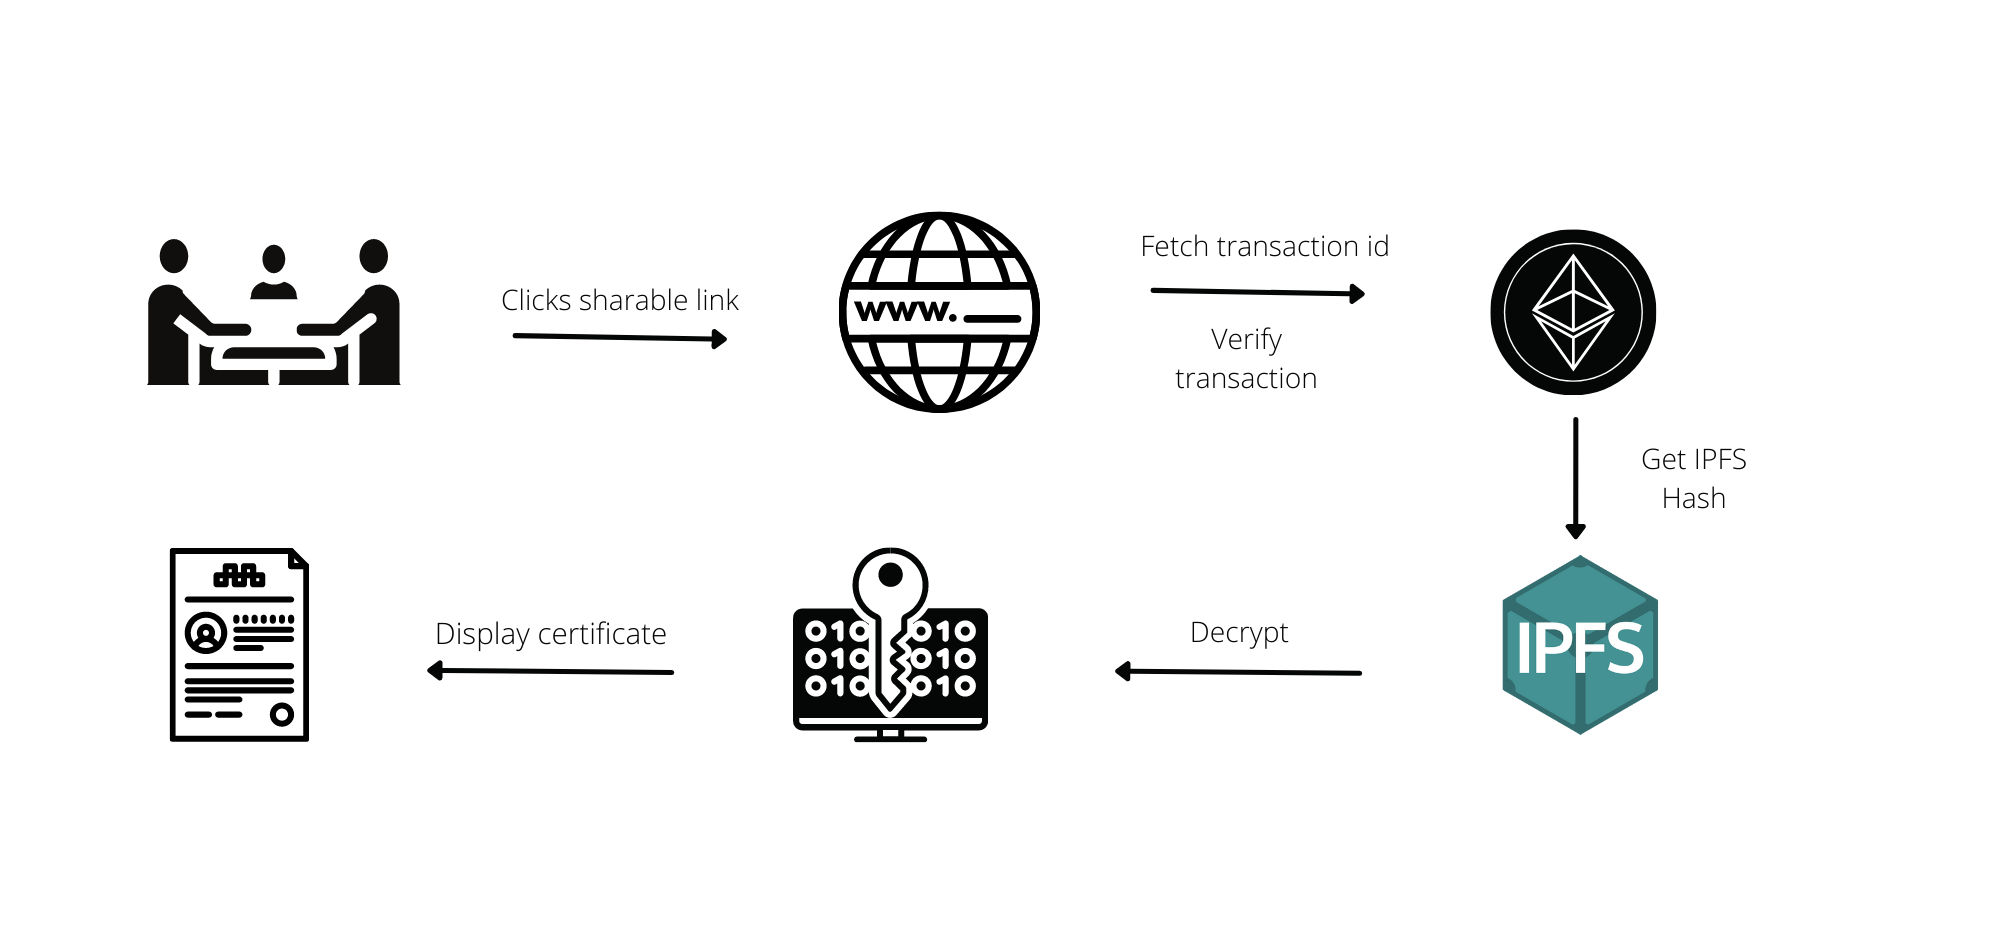
\includegraphics[width=\textwidth]{imgs/Third_party.png}
            \caption{Third Party module of the project}
            \label{fig:Third Party module of the project}
            \end{figure}